\section{Ziel}
Das Ziel des Versuches ist es, die Bragg Bedingung zu überprüfen, das Emissionsspektrum einer Cu-Röntgenröhre sowie das Absorptionsspektrum, bzw. die K-Kante und Abschirmungskonstante von fünf verschiedenen Materialien zu ermitteln.

\section{Theorie}
Röntgenstrahlung entsteht, wenn ein freies Elektron auf eine Anode einschlägt. Die Röntgenstrahlung eines Anodenmaterials ist durch ihre charakteristische Röntgenstrahlung sowie dem kontinuierlichen Bremsspektrum dessen charakterisiert. Bremsstrahlung entsteht durch die Wechselwirkung zwischen dem Elektron und dem Atomkern. Dabei wird ein Photon, auch Röntgenquant genannt, vom Elektron emittiert. Da das Elektron seine ganze Energie abgeben kann, ist das Bremsspektrum kontinuierlich. Wenn das Elektron vollständig gebremst wird, wandelt sich die kinetische Energie $E_{Kin}=eU$ in Strahlungsenergie $E=h\nu$ um. Die maximale Energie des Elektrons ergibt sich dann aus 
\begin{equation}
  \lambda_{min}=\frac{h\cdot c}{E},
  \label{1}
\end{equation}
der minimalen Wellenlänge.\\
Das charakteristische Spektrum ergibt sich daraus, dass das Anodenmaterial ionisiert wird und dann ein Elektron einer äußeren Schale in die innere Schale wandert, also in einen energetisch niedrigeren Zustand wechselt. Dadurch muss wieder ein Röntgenquant emittiert werden, dessen Energie sich aus der Energiedifferenz 
\begin{equation}
  h\nu=E_{m}-E_{n}
  \label{2}
\end{equation}
der beiden Energieniveaus ermitteln lässt. Diese signifikanten Sprünge ergeben das charakteristische Spektrum des Anodenmaterials, die als scharfe Linien dargestellt werden können. Diese Linien werden mit $K_{\alpha}, K_{\beta}, L_{\alpha}, ...$ bezeichnet, wobei $K,L,M,...$ für die jeweilige Schale steht. Dabei stehen griechische Buchstaben für die Herkunft des äußeren Elektrons, dass in die innere Schale wechselt. In einem Mehrelektronenatom schirmen die Hüllenelektronen die Elektronen der unteren Schalen ab. Dadurch wechselwirkt das äußere Elektron schwächer mit dem Kern und die Bindungsenergie, also die Energie, die benötigt wird, um das Elektron von der n-ten Schale des Atoms zu lösen beträgt
\begin{equation}
  E_{n}=-R_{\infty}z_{eff}^2\cdot\frac{1}{n^2},
  \label{3}
\end{equation}
wobei die Abschirmung in der effektiven Kernladung $z_{eff}=z-\sigma$ enthalten ist, mit der Abschirmkonstante $\sigma$ und der Rydbergenergie $R_{\infty}=13.6\ \si{\eV}$.\\
Zusätzlich können noch der Bahndrehimpuls und der Spin der äußeren Elektronen betrachtet werden. Dabei spaltet sich die charakteristische Kennlinie auf. Diese neue Struktur wird Feinstruktur genannt. Diese kann durch die Sommerfeldsche Feinstrukturformel 
\begin{equation}
  E_{n,j}=-R_{\infty}\left(z^2_{eff,1}\cdot \frac{1}{n^2}+\alpha^2 z^4_{eff,2}\cdot\frac{1}{n^3}\left(\frac{1}{j+\frac{1}{2}}-\frac{3}{4n}\right)\right)
  \label{4}
\end{equation}
berechnet werden, mit der Rydbergenergie $R_{\infty}$, der Feinstrukturkonstante $\alpha$, der effektiven Kernladungszahl $z_{eff}$, der Energiequantenzahl $n$ und dem Gesamtdrehimpuls $j$ des Elektrons.
Bei einer Röntgenstrahlung unter $1\ \si{\MeV}$ sind bei der Absorption der Comptoneffekt und der Photoeffekt relevant. Der Absorptionskoeffizient nimmt mit steigender Energie ab und springt, wenn die Photonenergie größer als die Bindungsenergie des Elektrons der nächsten inneren Schale ist. Die Energien der Elektronen 
\begin{equation}
  h\nu_{abs}=E_{n}-E_{\infty},
  \label{5}
\end{equation}
die aus den Schalen $K,L,M,...$ stammen, werden Absorptionskanten genannt. Bei der K-Kante gibt es nur eine Kante, bei L jedoch mehr. In der K-Schale ist $n=1$ und aus der Sommerfeldschen Feinstrukturformel lässt sich die Abschirmkonstante 
\begin{equation}
  \sigma_{K}=Z-\sqrt{\frac{E_{K}}{R_{\infty}}-\frac{\alpha^2 Z^4}{4}}
  \label{eq:6}
\end{equation}
berechnen.\\
Zuletzt lässt sich auch die Wellenlänge der Röntgenstrahlung aus der Bragg-Bedingung
\begin{equation}
  2dsin\theta=n\lambda
  \label{7}
\end{equation}
bestimmen, mit dem Glanzwinkel $\theta$, der gebeugten Wellenlänge $\lambda$ und der Beugungsordnung $n$. Das funktioniert, weil das Röntgenlicht an der Netzebene des Kristalls beugt, aber nur mit dem selben Wellenvektor $\vec k$ austreten kann, wenn es konstruktiv interferieren soll, heißt $\vec p=\hbar\vec k=\hbar\vec k'=\vec p'$, mit $\vec p$ Impuls der einlaufenden Welle und $\vec p'$ Impuls der auslaufenden Welle. 

\section{Versuchsaufbau}
\begin{figure}[H]
\centering
  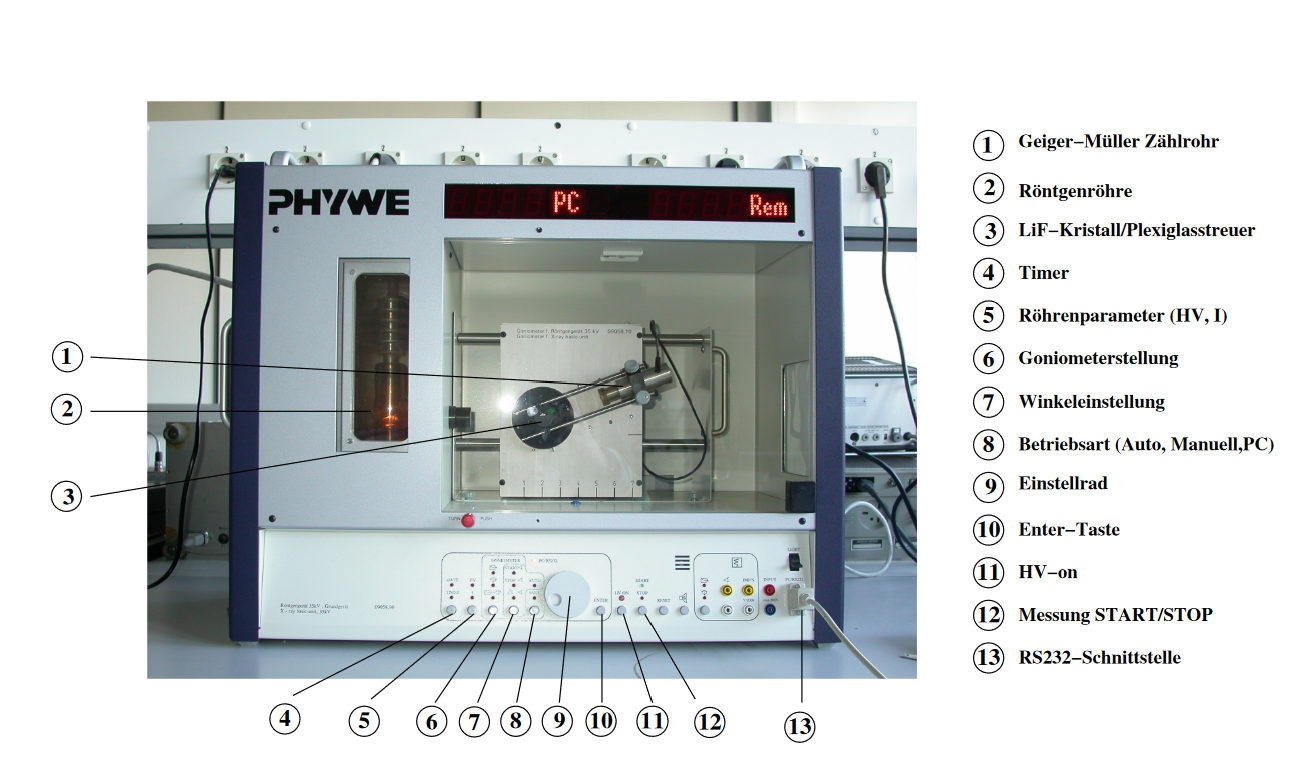
\includegraphics[width=9cm]{content/1.png}
  \caption{Das Messgerät}
  \label{fig:1}
\end{figure}
Für das Experiment wird lediglich eine Kuper-Röntgenröhre, ein KBr-Kristall und ein Geiger-Müller-Zählrohr benötigt. Das alles ist in dem Gerät aus \autoref{fig:1} geschaltet und kann über einen Rechner gesteuert werden. Die Beschleunigungsspannung wird auf $U=35\ \si{\keV}$ und der Emissionsstrom auf $I=1\ \si{\mA}$ gestellt.

\subsection{Überprüfung der Bragg-Bedingung}
Der KBr-Kristall wird auf einen festen Winkel von $\theta=14^{\circ}$ gestellt. Dann soll das Geiger-Müller-Zählrohr den Winkelbereich zwischen $\alpha_{1}=26^{\circ}$ und $\alpha_{2}=30^{\circ}$ in $\Delta\alpha=0.1^{\circ}$-Schritten mit einer Integrationszeit von $\Delta t=5\ \si{\s}$ pro Winkel die Intensität messen.

\subsection{Emissionsspektrum einer Cu-Röntgenröhre}
Zum Messen des Emissionsspektrums einer Cu-Röntgenröhre wir das Programm auf den 2:1 Koppelmodus gestellt und dann das Röntgenspektrum der Beugungsordnung $n=1$ im Winkelbereich zwischen $4^{\circ}\leq\theta\leq 26^{\circ}$ in $\Delta\alpha=0.2^{\circ}$-Schritten mit Integrationszeit $\Delta t=5\ \si{\s}$ gemessen. 

\subsection{Absorptionsspektrum}
Es sollen fünf Absorber mit Kernladungszahlen $30\leq Z\leq 50$ vor das Geiger-Müller-Zählrohr gesetzt werden und das Absorptionsspektrum in $\Delta\alpha=0.1^{\circ}$-Schritten mit Integrationszeit $\Delta t=20\ \si{\s}$ gemessen werden. Der Winkelbereich ist variabel.

\section{Vorbereitung}
Zur Vorbereitung sollte ermittelt werden, bei welchen Energien in keV die $\mathbf{Cu}-K_{\alpha}$- und $\mathbf{Cu}-K_{\beta}$-Linie zu erwarten ist. Diese liegen bei $E_{\mathbf{Cu}-K_{\alpha}}=8.05 \si{\keV}$ und $E_{\mathbf{Cu}-K_{\beta}}=8.91 \si{\keV}$. Die Glanzwinkel errechnen sich unter der Benutzung von \eqref{1} und \eqref{7} zu $\theta_{\alpha}=13.5^\circ$ und $\theta_{\beta}=12.2^\circ$.
Zusätzlich dazu sollte von Zn, Ge, Br, Rb, Sr und Zr die Absorptionskanten $E_{K}$, der Glanzwinkel $\theta_{K}$ und die Abschirmkonstante $\sigma_{K}$ gefunden werden:
\begin{table}[H]
  \centering
  \begin{tabular}{l|l|l|l|l}
  & Z & $E_{K}$ [keV] & $\theta_{K}$ [$^{\circ}$] & $\sigma_{K}$ \\\hline
  Zn & $30$ & $9.65$ & $11.3$ & $3.56$\\\hline
  Ge & $32$ & $11.10$ & $9.8$ & $3.68$\\\hline
  Br & $35$ & $13.47$ & $8.0$ & $3.85$\\\hline
  Rb & $37$ & $15.80$ & $7.1$ & $3.94$\\\hline
  Sr & $38$ & $16.10$ & $6.7$ & $3.99$\\\hline
  Zr & $40$ & $18.00$ & $6.0$ & $4.09$\\\hline
  \end{tabular}
  \caption{Stoffe, deren Ordnungszahlen, Absorptionskanten, Glanzwinkel und Abschirmkonstanten.}
  \label{tab:1}
\end{table}
